\documentclass{beamer}

\usepackage{default}
\usepackage[utf8]{inputenc}
\usepackage{tikz}
\usetikzlibrary{shapes,arrows,decorations,shapes}
\author{João Valença\\valenca@student.dei.uc.pt}
\institute{Department of Informatics Engineering\\University of Coimbra}
\date{February 2, 2015}
\subject{Theoretical Computer Science}
\title{Visualisation and Analysis of Geographic Information}
\subtitle{Algorithms and Data Structures}

\setbeamertemplate{navigation symbols}{}
\addtobeamertemplate{navigation symbols}{}{%
	\usebeamerfont{footline}%
	\usebeamercolor[fg]{footline}%
	\hspace{1em}%
	-- \insertframenumber\ --
}

\begin{document}
\frame{
	\titlepage
}
\frame{
	\frametitle{Motivation}
	\begin{itemize}
		\item Reduce visual information when displaying large numbers of geographic points
		\item Find a representative subset of a collection of geographic points
		\begin{figure}[H]
	\centering
	\begin{minipage}{0.4\linewidth}
		\centering
		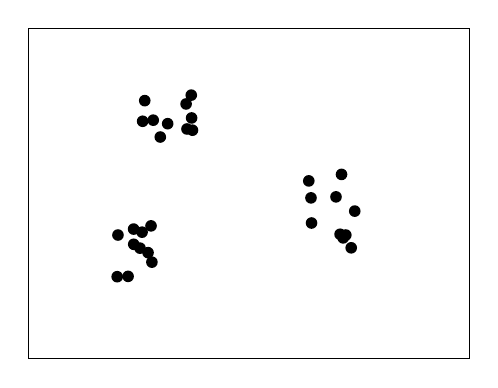
\begin{tikzpicture}[scale=1.4]
			\draw (-0.5,-0.4) rectangle (3.5,2.6);
			
			\fill (0.456,0.778)circle (1.5pt);
			\fill (0.622,0.478)circle (1.5pt);
			\fill (0.457,0.64)circle (1.5pt);
			\fill (0.614,0.807)circle (1.5pt);
			\fill (0.314,0.724)circle (1.5pt);
			\fill (0.533,0.75)circle (1.5pt);
			\fill (0.514,0.605)circle (1.5pt);
			\fill (0.307,0.346)circle (1.5pt);
			\fill (0.406,0.349)circle (1.5pt);
			\fill (0.587,0.564)circle (1.5pt);
			
			\fill (2.065,1.061)circle (1.5pt);
			\fill (2.045,1.215)circle (1.5pt);
			\fill (2.292,1.07)circle (1.5pt);
			\fill (2.381,0.724)circle (1.5pt);
			\fill (2.43,0.608)circle (1.5pt);
			\fill (2.342,1.274)circle (1.5pt);
			\fill (2.329,0.731)circle (1.5pt);
			\fill (2.462,0.941)circle (1.5pt);
			\fill (2.357,0.698)circle (1.5pt);
			\fill (2.07,0.833)circle (1.5pt);
			
			\fill (0.765,1.734)circle (1.5pt);
			\fill (0.557,1.943)circle (1.5pt);
			\fill (0.698,1.613)circle (1.5pt);
			\fill (0.634,1.766)circle (1.5pt);
			\fill (0.979,1.993)circle (1.5pt);
			\fill (0.99 ,1.675)circle (1.5pt);
			\fill (0.538,1.756)circle (1.5pt);
			\fill (0.932,1.913)circle (1.5pt);
			\fill (0.982,1.786)circle (1.5pt);
			\fill (0.94 ,1.686)circle (1.5pt);
		\end{tikzpicture}
		\caption*{\footnotesize Original Set}
		\label{fig:badrep}
	\end{minipage}
	\hspace{1cm}
	\begin{minipage}{0.4\linewidth}
		\centering
		\begin{tikzpicture}[scale=1.4]
		\draw (-0.5,-0.4) rectangle (3.5,2.6);
		
		\fill (0.765,1.734)circle (1.5pt);
		\fill (0.514,0.605)circle (1.5pt);
		\fill (2.292,1.07)circle (1.5pt);
		\end{tikzpicture}		
		\caption*{\footnotesize Representative Subset}
		\label{fig:goodrep}
	\end{minipage}
	\caption{Example of a Representative Set}
	\label{fig:rep}
\end{figure}
	\end{itemize}
	
}

\frame{
	\frametitle{}	
}

\end{document}
